\section{Fire !(50pts)}
Naviya在练习她的玫瑰礼花炮弹,她首先测试一下低功率火力的情况,她选择了一块平地作为测试场地。已知重力加速度为\(g\),炮弹的初速度为\(v_{0}\)。
\begin{enumerate}
	\item 如图\ref{fire1} 所示,Naviya发现她的炮弹的轨迹是抛物线,并且无意中发现似乎发射点到抛物线的焦点的距离一直是一个定值,并且还发现抛物线的准线一直没有发生改变,请你帮她证明这现象的正确性。(10pts)
	\begin{figure}[htbp]
	\centering
	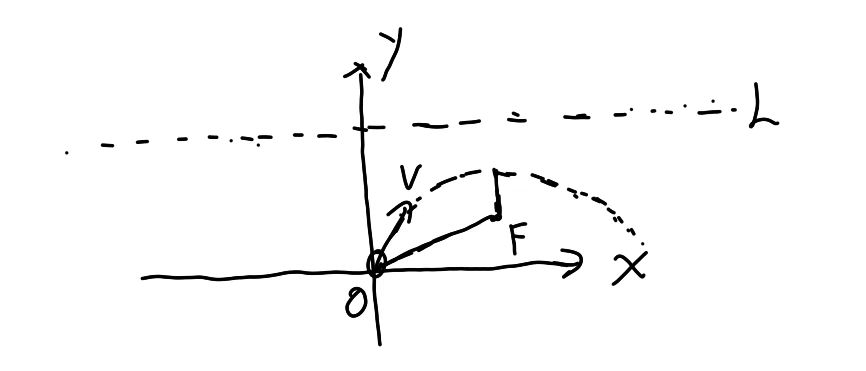
\includegraphics[width=0.5\textwidth]{fire1}
	\caption{炮弹轨迹示意图.}
	\label{fire1}
	\end{figure}
	\item 接着她想测试一下她的范围在限定的速度下能达到的最远的范围,也就是需要求出所有的抛物线的包络线,她猜测包络线也是一个抛物线,也就是对于任意轨迹上的任意一点P,到某一个点的距离始终小于或等于(可以取到等号)到某一条直线的距离。请你帮她找到这个点和这个直线,并且证明她的猜测是正确的,在写出包络线方程。(推荐几何方法解题哦,不过你也可以直接数学解析爆算但可能对下面题没有启发性)(10pts)
	\item 接着她开始加大炮塔的功率,使得炮弹的速度可以飞向太空中,但并没有超过第二宇宙速度。如图\ref{fire2}所示,她发现此时炮弹的轨迹变成了椭圆,她想知道现在发射点到焦点的距离是否还是一个定值?论证你的结论并帮她求出此时能达到的所有范围的包络线方程。(已知万有引力常数为\(G\),地球质量为\(M\),地球半径为\(R\),坐标原点设在地球中心,此问你可以不用考虑地球的碰撞体积)(20pts)
	\item 定义Naviya炮弹最小速度为使得第三问中的包络线恰好与地球表面相切的速度大小,求出这个速度的表达式。(10pts)
	\item 思考题:如果Naviya炮弹的速度超过了第二宇宙速度,那么包络线又会是什么?(0pts)
	\begin{figure}[htbp]
	\centering
	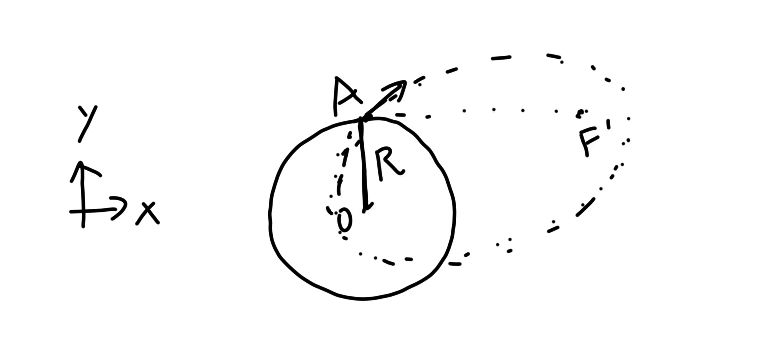
\includegraphics[width=0.5\textwidth]{fire2}
	\caption{炮弹轨迹示意图.}
	\label{fire2}
	\end{figure}
\end{enumerate}

\section*{Answer 2}
\begin{enumerate}
	\item 不难得到当以角度\(\theta\)发射炮弹时,炮弹的运动方程为:
	\begin{align*}
		x(t) &= v_0 \cos \theta t \\
		y(t) &= v_0 \sin \theta t - \frac{1}{2}gt^2
	\end{align*}
	将\(t\)消去,得到抛物线方程为:
	\begin{align*}
		y &= \frac{g}{2v_0^2 \cos^2 \theta} x^2 - \tan \theta x
	\end{align*}
		我们可以看到,抛物线的半正交弦为\(p=\frac{v_0^2 \cos^2 \theta}{g}\), 
		焦点坐标为:
	\begin{align*}
			F_x &= \frac{v_0^2 \sin2 \theta}{2g} \\
			F_y &= -\frac{v_0^2 \cos2 \theta}{2g}
	\end{align*}
	OF的距离为一个定值:
	\begin{align*}
		OF &= \sqrt{F_x^2 + F_y^2} \\
		   &= \frac{v_0^2}{2g} \sqrt{\sin^2 2\theta + \cos^2 2\theta} \\
		   &= \frac{v_0^2}{2g}
	\end{align*}
		而抛物线的准线为:
	\begin{align*}
		y &=h + \frac{p}{2} \\
		h &= \frac{v_0^2 \sin^2 \theta}{2g} \\
		p &= \frac{v_0^2 \cos^2 \theta}{g} \\
		y &= \frac{v_0^2}{2g} 
	\end{align*}
	\item 如图\ref{fire1a}所示,设点\(P\)为抛物线上的任意一点,点\(F\)为焦点,构造一条新的直线\(L_2\),它与抛物线准线的距离恰好为\(\Delta = OF = \frac{v_0^2}{2g}\).
	\begin{figure}[htbp]
	\centering
	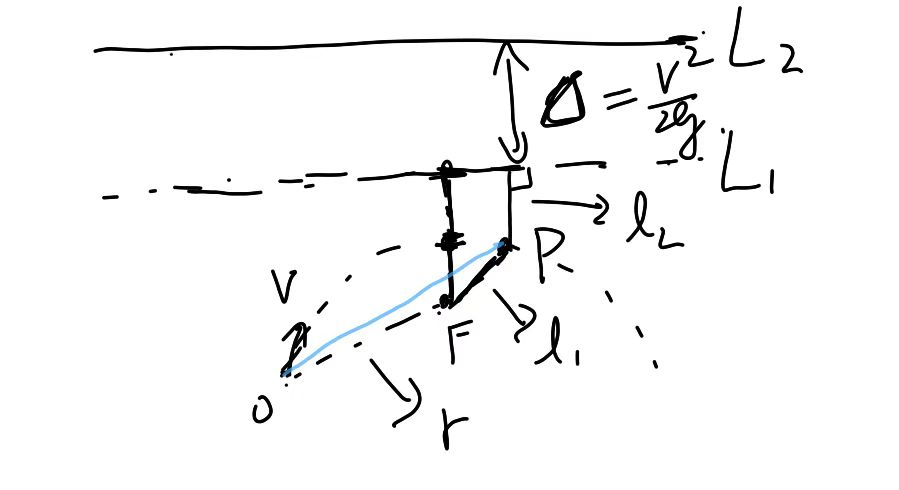
\includegraphics[width=0.5\textwidth]{fire1a}
	\caption{炮弹轨迹示意图.}
	\label{fire1a}
	\end{figure}
		我们可以看到
	\begin{align*}
		OP &\leq OF + l_1=\Delta +l_2 
	\end{align*}
	于是我们看到,OP始终小于等于到\(L_2\)的距离,并且可以取到等号。
		所以包络线就是一条抛物线,焦点为原点O,准线为\(L_2\).对应的\(p'=\Delta=\frac{v_0^2}{2g}\)方程为:
	\begin{align*}
		x^2=-2p'(y-p')  
	\end{align*}
	\item 首先我们计算半长轴\(a\),
	由能量:
	\begin{align*}
		E = \frac{1}{2}mv_0^2 - \frac{GMm}{R} = -\frac{GMm}{2a} \\
		a = -\frac{GM}{2E} = \frac{GMR}{2GM - v_0^2R}
	\end{align*}
	作图如下:
	\begin{figure}[htbp]
	\centering
	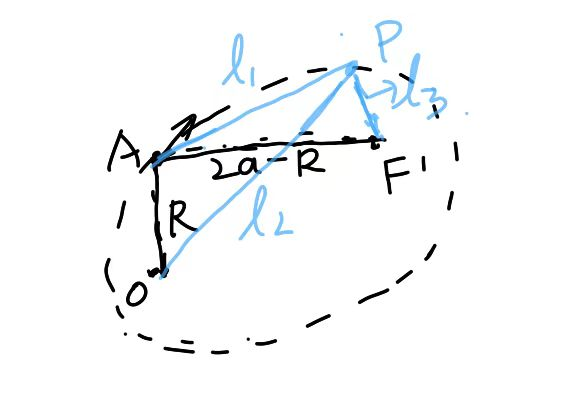
\includegraphics[width=0.5\textwidth]{fire2a}
	\caption{炮弹轨迹示意图.}
	\label{fire2a}
	\end{figure}
		我们可以看到,炮弹的轨迹是一个椭圆,焦点为\(O,F'\),我们有:
	\begin{align*}
		AF' = 2a - R
	\end{align*}
	也为一个定值!(这也说明椭圆的另一个焦点的轨迹是一个圆,但这一点性质并没有什么用。)我们又有\(l_2+l_3=2a\),
	从而:
	\begin{align*}
		l_1+l_2\leq  (AF' + l_3) + l_2 = AF' + 2a = 4a - R
	\end{align*}
	恒小于等于一个定值,并且可以取到等号。
		所以包络线就是一条椭圆,焦点为\(O,A\),半长轴为\(A=2a-\frac{R}{2}\),半焦距为\(C=\frac{R}{2}\),半短轴为\(B=\sqrt{a^2-c^2}\),注意坐标原点为O, 故Naviya包络线方程为:
	\begin{align*}
		\frac{x^2}{(2a-\frac{R}{2})^2} + \frac{(y-\frac{R}{2})^2}{(2a-\frac{R}{2})^2-(\frac{R}{2})^2} = 1
	\end{align*}
	\item 与地球方程联立:
	\begin{align*}
		\frac{x^2}{(2a-\frac{R}{2})^2} + \frac{(y-\frac{R}{2})^2}{(2a-\frac{R}{2})^2-(\frac{R}{2})^2}  &= 1 \\
		x^2 + y^2 &= R^2
	\end{align*}
	消去\(x\),令\(Y=\frac{y}{R}\),\(\lambda = \frac{A}{R}\),我们有:
	\begin{align*}
		Y^2 -4Y\lambda^2+2\lambda^2-1 &= 0 
	\end{align*}
	要求相切,则要求只能恰好有一个\(Y\)的解,判别式为:
	\begin{align*}
		\Delta &= 16\lambda^4 - 8\lambda^2 + 4 =0
	\end{align*}
		我们可以得到:
	\begin{align*}
		\lambda = \frac{\sqrt{1+\sqrt{5}}}{2}
	\end{align*}
	于是我们可以得到Naviya炮弹的最小速度为:
	\begin{align*}
		a &= \frac{1+\sqrt{1+\sqrt{5}}}{4}R \\
		v_{Naviya} &= \sqrt{\frac{GM}{R}(2-\frac{4}{1+\sqrt{1+\sqrt{5}}})} 
	\end{align*}

\end{enumerate}